\subsection*{Local minima}
    
    Even if we don't have that problem, we have a \textbf{different} one:
    
    Gradient descent \textbf{gradually} improves our solution until it reaches one it's \textbf{satisfied} with. But, what if there are \textbf{multiple} solutions we could reach?
    
    Are they all equally good?
    
    \begin{figure}[H]
    \centering
        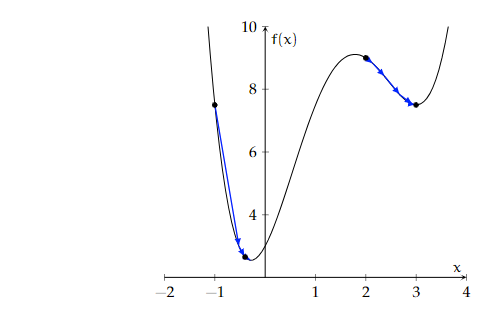
\includegraphics[width=70mm,scale=0.5]{images/gradient_descent_images/Two_Local_Minima.png}
    
    \caption*{Depending on your starting position (\textbf{initialization}), you could find a different local minimum!}
    \end{figure}
    
    Maybe not! So, if our function isn't \textbf{always convex}, we can end up with \textbf{multiple} "valleys", or \textbf{local} minima.\\
    
    \begin{definition}
        A \vocab{global} minimum is the \purp{lowest} point on our entire function: the one with the lowest \gren{output}.
        
        A \vocab{local} minimum is one that is the \gren{lowest} point among those points that are \purp{near} it.
        
        \begin{itemize}
            \item For \vocab{local minima}, if you add or subtract a \purp{small} amount $\epsilon$, the value will \gren{increase}.
        \end{itemize}
        
    \end{definition}
    
    So, we \textbf{won't} necessarily end up with the \textbf{global} minimum, even with a \textit{small} $\eta$.
    
    This shows that \textbf{initialization matters}!\\
    
    \begin{definition}
        \vocab{Initialization} is our "starting point": when we first \gren{start} our algorithm, what are our \purp{parameters} set to?
    \end{definition}
    
    If we have a \textbf{different} starting position, we can find a \textbf{different} local minimum.\\
    
    \begin{concept}
        \vocab{Gradient descent} finds \purp{local} minima near the initialization, not \purp{global} minima.
        
        This means, if our function has \vocab{multiple local minima} (not fully convex), our \vocab{initialization} can affect our \gren{solution}.
    \end{concept} 